%% kolla att allt �r i imperfekt
%% verb i passiv form

\section{Existing verification tools}
Software unit testing can be achieved by almost any tool.
%% motivera.
Consequently this phase is not the most interesting when it comes to the choice
of a tool verification. Of course one can take the simplicity to achieve good
%% "simplicity" - av vad?
unit testing into account, but still it is not what makes a verification tool
especially unique for the project goals.

Since the purpose is about benchmarking software the phase ``verification of
%% what now? Introduce ISO-phases!
software safety requirements'' will not influence the choice. To be able to test
this phase, a greater amount of components of the whole system must be
available. Such components include hardware, and this report will not cover
hardware integration. The implementation should be able to run on a standard
PC-machine.

The most interesting part is the phase ``software integration and testing''. Is there a
tool that one can use to easily combine test and requirements from different
modules? Is it possible to test functional safety concept from this
combination, for example by corrupting some software elements?

%% SKRIV OM vilka delar i ISO~26262 vi kan testa mha Quickcheck (6-9, 6-10,
%% 6-11)

% \subsection{CORE}
% A specification package developed by British Aerospace and System Designers.

%\subsection{Promela}

\subsection{SPIN}
SPIN is used to trace logical design errors in distributed
software\cite{SPIN:manual}. It supports a high level language, Promela, to
specify system descriptions. Promela is an acronym for PROcess MEta LAnguage, and
is a verification model language. The system properties that should be checked
are written in logical temporal language (LTL), and SPIN reports errors such as
deadlocks, race conditions and incompleteness between these properties and the
system model. It also supports embedded C code as part of the model
specifications. It supports random, interactive and guided simulation, with both
partial and exhaustive proof techniques.

% \subsection{McErlang}
% McErlang is a model checker written in Erlang used for verifying distributed
% Erlang programs\cite{MCERLANG:model-checker}. Its purpose is to check a program
% against a correctness property, but can also among other things check safety
% or liveness properties.

% McErlang offers two depth-first state traversal model checking algorithms; one
% checks safety properties and the other is used for checking the liveness
% properties. McErlang also implements weak process fairness, by omitting non-fair
% loops from the accepting runs in its liveness algorithm.

% %% jag tror mcerlang ing�r i QuickCheck suiten. den blir installerad tillsammans
% %% med QuickCheck iaf.

\subsection{$\mu$CRL toolset} $\mu$CRL is a process algebraic language which is
suited for the analysis of distributed systems. The toolkit is built on this
language and contains a theorem prover based on binary decision
diagrams\cite{MCRL:manual}.

\subsection{CADP} Construction and Analysis of Distributed Processes (CADP),
formerly CAESAR/ALDEBARAN Development Package, is a toolset for the design of
distributed systems\cite{CADP:manual}. It includes, among others, tools for
equivalence checking, state-space manipulation and model checking, and it also
includes several verification algorithms. It provides functionality as
step-by-step simulation to parallel model checking.

\subsection{Parasoft C++test}
Parasoft C++ is a commercial software with a huge range of functionality,
developed by the Parasoft company, with the purpose of testing software written
in C or C++. Parasoft claims that it should be possible to satisfy ASIL
requirements using their software(?).
%\subsection{Isabelle}
% Isabelle theorem prover is an interactive theorem prover, successor of the
% Higher Order Logic (HOL) theorem prover

%% \subsection{Why QuickCheck and Erlang?}

\section{Specification}
In AUTOSAR, specifications for each module is given in text form. Consequently
one must first, before a module can be tested, implement the specification for
that module in code.

\section{Testing}
%% vilka properties? quickcheck?
%% kanske �r b�ttre att skriva "Module properties have to take..."
%% alternativt "Quickcheck properties for a module have to take..."
Properties for a module have to take the current state in consideration, since
most functions written in an imperative language are not immutable. This gives
raise to the idea of a state based testing tool.
%% .. och pl�tsligt: en lista:...
\begin{itemize}
\item Choose a specification which will be translated to QuickCheck properties
in parts.
\item With the use of statistics, show that, with enough tests the state-space
  will be exhausted.
\item Evaluate other semi formal techniques and show that the results from them
shows that QuickCheck is reliable for verification.
\item Generalize the technique.
\end{itemize}

\section{Choice of AUTOSAR module to test}
There were several modules that were up for discussion when it came to the
choice of a module to test. Since the goal was to get a proof of concept for
that it was possible to
get an ASIL-classification and achieve functional safety using Quickcheck, it
seemed preferable to choose a less complicated module. It was also desirable to
have the actual C code and not just library files.

\section{Implementation}
The C-code that was to be tested, using QuickCheck, was already unit tested and
run sharp in lab environments.

The WdgM model was completely implemented in Erlang, independent of the design
choices of the C-code. The idea was to ensure an independent model; if the model
was inspired by the C-code, it could have transmitted errors.

The implementation of the module was done to be able to test API calls,
also described in appendix~\ref{APP:QUICKCHECK}, against the C-code. The tests
then checked that the postconditions held, according to figure
\ref{FIG:api_calls}. The postconditions were written to test that AUTOSAR
requirements held. In other words that the API calls were called correctly. A
problem when writing the postconditions, was to translate the AUTOSAR
requirements into code, because AUTOSAR specification are written in natural
language. It was easy to see that there were room for different interpretations,
which most likely would
result in errors later.

The implementation of the AUTOSAR module in Erlang was done
in an iterative way. Every piece of code were not required to be implemented before
tests could be run. This because of that a module in AUTOSAR consist of several API
calls. It was enough to implement some specification for one API call
before tests could be run. Of course this gave rise to that only a part of
the C-code was tested. Also early tests may not have fully tested the
implemented API call because some branches in the C-code will never have been
reached before other unimplemented API calls.

\begin{figure}[!h]
\begin{center}
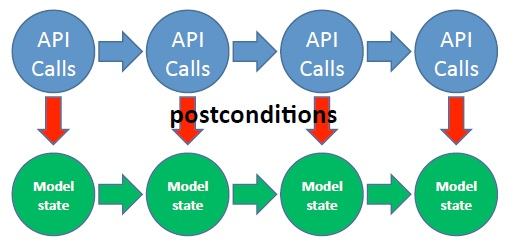
\includegraphics{pictures/api_calls.jpg}
\end{center}
\caption{Shows Erlang modeled states with calls against the C-code}
\label{FIG:api_calls}
\end{figure}
Early in the implementation phase Quickcheck found differences between the Erlang
and C-implementation. This was expected because every programmer makes mistakes.
The question was whether the fault was in the C-code or the Erlang code. Then
the API was thoroughly read and a conclusion was made. Either a bug in the
C-code was found or the Erlang-code needed to be corrected. There were however
cases when the API was ambiguous. In those cases the C-interpretation was chosen
as correct and the ambiguous specification written down.

Surprisingly bugs in the C-code was found early, even though it already run
sharp in lab environments; only a few specification requirements needed to be
implemented in Erlang.

If a bug in the C-code was discovered how should the work be continued? Since
Quickcheck terminates as soon as it finds a counter example something was needed to
be able to run further tests. Some alternatives were discussed.

\begin{enumerate}
        \item Fix the C-code, in other words change the C source code.
                \label{ENUMERATE:FixCCode}
        \item Mocking, in other words simulate different C-code output.
        \item Change the Erlang module to a faulty behavior to follow the C
                implementation.
\end{enumerate}

Item \ref{ENUMERATE:FixCCode} was chosen, see section \ref{sec:handlebugs}.

When thoroughly reading the AUTOSAR API not only ambiguous rules were found but
also rules that contradicted each other were recognized. In those cases the
implementation in the C-code was followed.

A great tool when a clear interpretation of the AUTOSAR specification was not
possible was to look into the C-code. Even though Quickcheck can be used to
test libraries when the actually source code is not available.

When the full module was implemented in Erlang code there had to be some assurance
for that every piece of code in the C implementation was actually tested.
Code coverage for the Erlang implementation was measured using the Erlang module
\emph{cover}. To be able to to measure the code coverage of the C-code the
commercial tool Bullseye Coverage was used. Only by using those tools it was
easy to see that the result was not good enough. The main problem seemed to be
that the WdgM was put in an absorbing state and after that following commands
did not test anything interesting. The reason for that an absorbing state was
reached was the availing of negative testing. The testing was negative because
invalid command sequences and arguments were generated.

Figure \ref{FIG:ONERUN} shows how the status of the watchdog manager changes
during the execution of API calls. After a number of commands the absorbing
state \emph{stopped} is reached.

\begin{figure}
  \begin{center}
    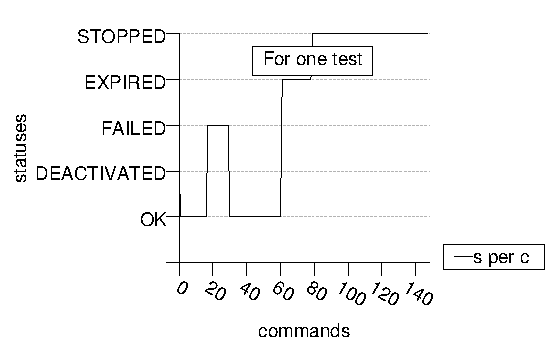
\includegraphics{generated_pictures/one_test_history_statuses_freescale.pdf}
    \caption{Shows how the status changes in the execution of one QuickCheck test}
    \label{FIG:ONERUN}
  \end{center}
\end{figure}

The next step was to tweak the generators, used by Quickcheck, to construct
valid API-calls. There were several branches in the C-code
that needed a specific sequence of API calls, with correct arguments, to be
reached. Also the tweaking of the generators could be implemented in a iterative
way. Change the probability properties of the generators and check the results.
The results were analyzed and the generators were tweaked even more to make the
results even better.

%% Just checking code coverage was however not good enough for our goals...

To get a better picture of the work flow used in this thesis see
figure \ref{fig:workflow}.

\begin{figure}[!ht]
\caption{Work flow}
\label{fig:workflow}
\fbox{
\parbox{\linewidth}{
\begin{enumerate}
\item Construct a model for an AUTOSAR module in Erlang
\item Run Quickcheck for this model and compare the results with the output from
the c code. \label{compare}
\item Tweak the generators for the test cases \label{generators}
    \item Evaluate the results
    \begin{enumerate}
      \item What is the state space?
      \item Which test cases are relevant?
      \item Collapse irrelevant states
      \item What can be said about the results?
    \end{enumerate}
\item Are the results good enough, does it satisfy the requirements for the ASIL
levels?
\item If not go the step \ref{compare}
\end{enumerate}
}}
\end{figure}
%even though correction of the C-code
%was not part of the thesis. Since there were actually code available, not
%only libraries, and most bugs was easy to fix this seemed like the best choice,
%see results.

A challenging step is the analysis of the results. If the testing tool returns zero
errors what does that say about the robustness of the input byte code? Passed
100 of 100 tests is just a statement and does not say anything more than that
some tests passed. Can tests be implemented in a clever way so that it is
possible to get some kind of confidence on the correctness of the code?

\section{Configurations}
When the code coverage was calculated it was recognized that every piece of code
wasn't executed. The reason seemed to be that the current configuration
disallowed, even though the program behaved correctly, the execution of those
lines of code. Because of that the implementation of the Erlang module was done
independent of configuration it was easy to to run tests on several
configuration which resulted in that everything was executed.

The tweaking of generators, to achieve better test cases, seemed in some sense to be
configuration dependent. Better test cases were generated if the generators were
tweaked according to a specific configuration, see results.

\begin{figure}[!ht]
% Graphic for TeX using PGF
% Title: /home/oskar/documents/box.dia
% Creator: Dia v0.97.2
% CreationDate: Sat Sep  7 19:28:43 2013
% For: oskar
% \usepackage{tikz}
% The following commands are not supported in PSTricks at present
% We define them conditionally, so when they are implemented,
% this pgf file will use them.
\ifx\du\undefined
  \newlength{\du}
\fi
\setlength{\du}{15\unitlength}
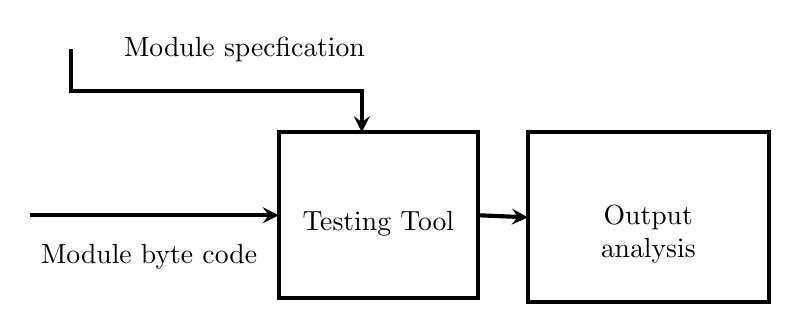
\begin{tikzpicture}
\pgftransformxscale{1.000000}
\pgftransformyscale{-1.000000}
\definecolor{dialinecolor}{rgb}{0.000000, 0.000000, 0.000000}
\pgfsetstrokecolor{dialinecolor}
\definecolor{dialinecolor}{rgb}{1.000000, 1.000000, 1.000000}
\pgfsetfillcolor{dialinecolor}
\definecolor{dialinecolor}{rgb}{1.000000, 1.000000, 1.000000}
\pgfsetfillcolor{dialinecolor}
\fill (6.000000\du,7.000000\du)--(6.000000\du,11.000000\du)--(10.795000\du,11.000000\du)--(10.795000\du,7.000000\du)--cycle;
\pgfsetlinewidth{0.100000\du}
\pgfsetdash{}{0pt}
\pgfsetdash{}{0pt}
\pgfsetmiterjoin
\definecolor{dialinecolor}{rgb}{0.000000, 0.000000, 0.000000}
\pgfsetstrokecolor{dialinecolor}
\draw (6.000000\du,7.000000\du)--(6.000000\du,11.000000\du)--(10.795000\du,11.000000\du)--(10.795000\du,7.000000\du)--cycle;
% setfont left to latex
\definecolor{dialinecolor}{rgb}{0.000000, 0.000000, 0.000000}
\pgfsetstrokecolor{dialinecolor}
\node at (8.397500\du,9.195000\du){Testing Tool};
\pgfsetlinewidth{0.100000\du}
\pgfsetdash{}{0pt}
\pgfsetdash{}{0pt}
\pgfsetbuttcap
{
\definecolor{dialinecolor}{rgb}{0.000000, 0.000000, 0.000000}
\pgfsetfillcolor{dialinecolor}
% was here!!!
\pgfsetarrowsend{stealth}
\definecolor{dialinecolor}{rgb}{0.000000, 0.000000, 0.000000}
\pgfsetstrokecolor{dialinecolor}
\draw (10.795000\du,9.000000\du)--(12.000000\du,9.050000\du);
}
\pgfsetlinewidth{0.100000\du}
\pgfsetdash{}{0pt}
\pgfsetdash{}{0pt}
\pgfsetbuttcap
{
\definecolor{dialinecolor}{rgb}{0.000000, 0.000000, 0.000000}
\pgfsetfillcolor{dialinecolor}
% was here!!!
\pgfsetarrowsend{stealth}
\definecolor{dialinecolor}{rgb}{0.000000, 0.000000, 0.000000}
\pgfsetstrokecolor{dialinecolor}
\draw (0.000000\du,9.000000\du)--(6.000000\du,9.000000\du);
}
% setfont left to latex
\definecolor{dialinecolor}{rgb}{0.000000, 0.000000, 0.000000}
\pgfsetstrokecolor{dialinecolor}
\node[anchor=west] at (8.397500\du,9.000000\du){};
% setfont left to latex
\definecolor{dialinecolor}{rgb}{0.000000, 0.000000, 0.000000}
\pgfsetstrokecolor{dialinecolor}
\node[anchor=west] at (0.000000\du,10.000000\du){Module byte code};
% setfont left to latex
\definecolor{dialinecolor}{rgb}{0.000000, 0.000000, 0.000000}
\pgfsetstrokecolor{dialinecolor}
\node[anchor=west] at (3.000000\du,8.000000\du){};
% setfont left to latex
\definecolor{dialinecolor}{rgb}{0.000000, 0.000000, 0.000000}
\pgfsetstrokecolor{dialinecolor}
\node[anchor=west] at (2.000000\du,5.000000\du){Module specfication};
\definecolor{dialinecolor}{rgb}{1.000000, 1.000000, 1.000000}
\pgfsetfillcolor{dialinecolor}
\fill (12.000000\du,7.000000\du)--(12.000000\du,11.100000\du)--(17.800000\du,11.100000\du)--(17.800000\du,7.000000\du)--cycle;
\pgfsetlinewidth{0.100000\du}
\pgfsetdash{}{0pt}
\pgfsetdash{}{0pt}
\pgfsetmiterjoin
\definecolor{dialinecolor}{rgb}{0.000000, 0.000000, 0.000000}
\pgfsetstrokecolor{dialinecolor}
\draw (12.000000\du,7.000000\du)--(12.000000\du,11.100000\du)--(17.800000\du,11.100000\du)--(17.800000\du,7.000000\du)--cycle;
% setfont left to latex
\definecolor{dialinecolor}{rgb}{0.000000, 0.000000, 0.000000}
\pgfsetstrokecolor{dialinecolor}
\node at (14.900000\du,9.245000\du){};
\pgfsetlinewidth{0.100000\du}
\pgfsetdash{}{0pt}
\pgfsetdash{}{0pt}
\pgfsetmiterjoin
\pgfsetbuttcap
{
\definecolor{dialinecolor}{rgb}{0.000000, 0.000000, 0.000000}
\pgfsetfillcolor{dialinecolor}
% was here!!!
\pgfsetarrowsend{stealth}
{\pgfsetcornersarced{\pgfpoint{0.000000\du}{0.000000\du}}\definecolor{dialinecolor}{rgb}{0.000000, 0.000000, 0.000000}
\pgfsetstrokecolor{dialinecolor}
\draw (1.000000\du,5.000000\du)--(1.000000\du,6.000000\du)--(8.000000\du,6.000000\du)--(8.000000\du,7.000000\du);
}}
% setfont left to latex
\definecolor{dialinecolor}{rgb}{0.000000, 0.000000, 0.000000}
\pgfsetstrokecolor{dialinecolor}
\node at (14.900000\du,9.050000\du){Output};
% setfont left to latex
\definecolor{dialinecolor}{rgb}{0.000000, 0.000000, 0.000000}
\pgfsetstrokecolor{dialinecolor}
\node at (14.900000\du,9.850000\du){ analysis };
\end{tikzpicture}

\caption{Abstract implementation module}
\end{figure}

\section{Calling the API commands}
\label{SEC:CALLING_COMMANDS}
API calls were executed by QuickCheck using the \emph{run\_commands/1} function
according to \ref{SEC:QuickCheckIntro}. The runtime environment module (RTE) is
however responsible for the scheduling of the main function, which should be
executed in a given time interval. Since the RTE was not available when testing
the watchdog manager the main function was called randomly and it was
assumed that every time the main function was called a given amount of time had
passed.

Except the main function only one internal algorithm used by the watchdog
manager was time dependent, namely deadline supervision. A deadline supervision
consist of two checkpoints. One start checkpoint, one stop checkpoint and a
maximum time it shall take to reach the stop checkpoint after the start
checkpoint was reached. The AUTOSAR specification was however lacking of a
clear definition of how time should be represented. The C code just used ticks,
not actual time stamp, which was incremented every time the main function was
called. It was in other words assumed that the RTE was able to execute the main
function correctly and a fixed amount of ticks would always represent the same
amount of time. Accepting this solution it was easy to adopt the same approach
in the Erlang module. More about this can be found in section
\ref{SEC:FUNCTIONAL_SAFETY_TIME}.

\section{Model State}
The model state was constructed as easy as possible. Hence, even though it was
attempting to use a more efficient data structure, a simple record was used to
represent the model state. The main reason for that was to make it easier to
follow the model state when for instance using
\emph{eqc\_statem:show\_states/1}, see appendix \ref{APP:QUICKCHECK}. The
efficiency of the test model was considered less relevant then the readability
of the model state.  The idea was to make it easy to find the actual bug, when
there were conflicts between the C-code and the Erlang module, and running the
actual tests was not considered time or memory critical.
